\documentclass[aspectratio=169]{beamer}

\usepackage[utf8]{inputenc}
%\usepackage{latexsym}
\usepackage{graphicx}
\usepackage{mathptmx}
\usepackage{amsmath}
%\usepackage{amsfonts}
\usepackage{amssymb}
\usepackage{amsbsy}
\usepackage{amsthm}
\usepackage{algorithmic}

% Get checkmark logo
\usepackage{pifont}
\newcommand{\cmark}{\ding{51}}
\newcommand{\xmark}{\ding{55}}
% Get \lee and \gee commands
\newcommand{\lee}{\leqq}
\newcommand{\gee}{\geqq}

% Strikouts
\usepackage[normalem]{ulem}

% Restore Mathcal
\let\saveboldmath\boldmath
\usepackage{mathptmx}
\let\boldmath\saveboldmath
\usepackage{bm}
\DeclareSymbolFont{cmsymbols}{OMS}{cmsy}{m}{n}
\SetSymbolFont{cmsymbols}{bold}{OMS}{cmsy}{b}{n}
\DeclareSymbolFontAlphabet{\mathcal}{cmsymbols}

\usepackage[english]{babel}
\usepackage[utf8]{inputenc}

% AMSLaTeX packages
\usepackage{amsthm}
\usepackage{amsmath}
\usepackage{amsfonts}
\usepackage[algoruled]{algorithm2e}

\usetheme{default}
\useoutertheme{default}
% we want to use images
\usepackage{graphicx}
\usepackage{movie15}
\usepackage{hyperref}

% table relates packages
\usepackage{booktabs}
\usepackage{multirow}
% pick a font
\usepackage{palatino}           
% \usepackage{times}
\usepackage{tikz}
\usetikzlibrary[positioning,arrows,decorations.pathmorphing,backgrounds,fit,calc]
% \AtBeginSection[]  % "Beamer, do the following at the start of every section"
% {
%   \begin{frame}<beamer> 
%     \frametitle{Outline} % make a frame titled "Outline"
%     \tableofcontents[currentsection]  % show TOC and highlight current section
%   \end{frame}                    
% }

% \AtBeginSubsection[]
% {
%   \begin{frame}
%     \frametitle{Outline}
%     \tableofcontents[currentsection,currentsubsection]
%   \end{frame}
% }

\AtBeginSection[]
{
   \begin{frame}
       \frametitle{Outline}
       \tableofcontents[currentsection]
   \end{frame}
}

\newcommand{\ebox}[1][1em]{\framebox[#1]{\phantom{M}}}

\setlength\arraycolsep{1.4pt}% some length

%gets rid of navigation symbols
\setbeamertemplate{navigation symbols}{}

%gets rid of bottom navigation bars
\setbeamertemplate{footline}[page number]{}
\setbeamertemplate{headline}{}


\usebackgroundtemplate{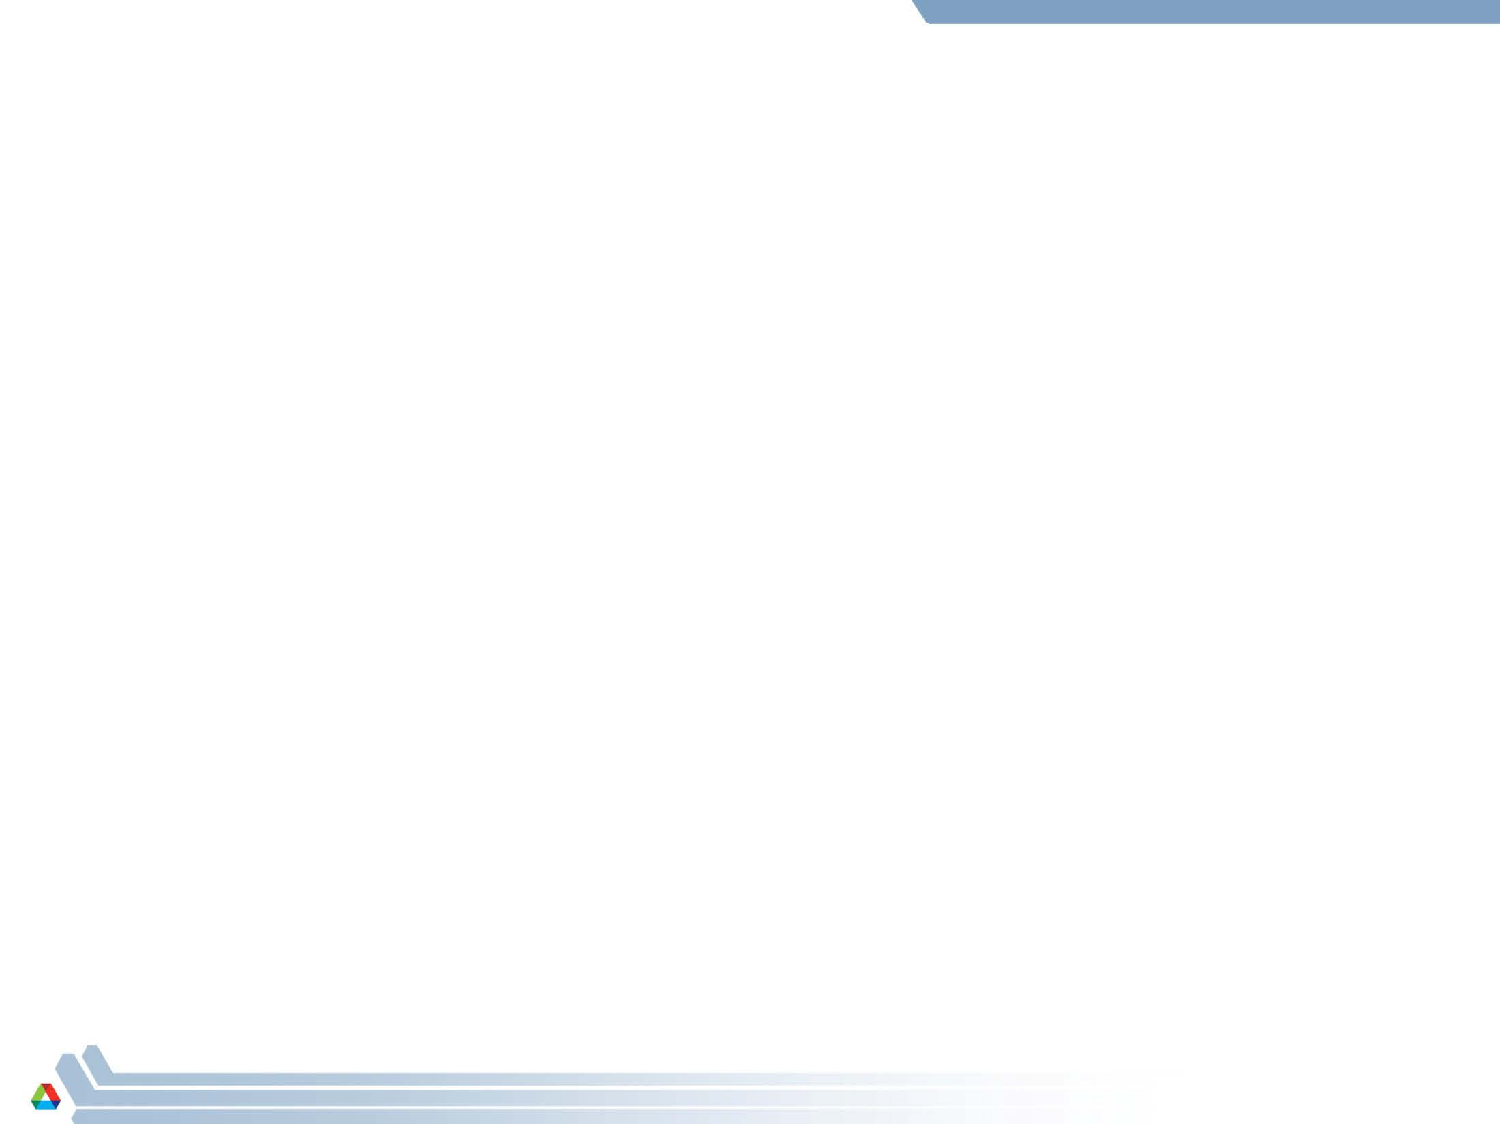
\includegraphics[width=\paperwidth]{../templates/NormalANLBlue}}
% Title Information
\title{Toward interpretable machine learning via Delaunay interpolation}
\subtitle{Algorithms and challenges}
\author{Tyler Chang}
\date{LANS Seminar Series\\
July 12, 2023}
\institute{Argonne National Laboratory}

\begin{document}

\setbeamertemplate{footline}{}
{
\usebackgroundtemplate{
\includegraphics[width=\paperwidth]{../templates/TitleANLBlue}}
\frame{\titlepage}
}

\setbeamertemplate{footline}[page number]{}

% FRAME: overview
\begin{frame}
  \frametitle{Outlines}
  \tableofcontents
\end{frame}

\section{Inference problems and high-dimensional modeling}

\begin{frame}\frametitle{The fundamental machine learning problem}

\begin{columns}
\begin{column}{0.5\textwidth}

\onslide<2>{
\begin{center}
\includegraphics[width=\textwidth]{../img/delaunay_new/inference_1d_pt1.eps}
\end{center}
}

\onslide<3>{
\begin{center}
\vskip -14.5em
\includegraphics[width=\textwidth]{../img/delaunay_new/inference_1d_pt2.eps}
\end{center}
}

\onslide<4>{
\begin{center}
\vskip -14.5em
\includegraphics[width=\textwidth]{../img/delaunay_new/inference_1d_pt3.eps}
\end{center}
}

\onslide<5>{
\begin{center}
\vskip -14.5em
\includegraphics[width=\textwidth]{../img/delaunay_new/inference_1d_pt4.eps}
\end{center}
}

\onslide<6>{
\begin{center}
\vskip -14.5em
\includegraphics[width=\textwidth]{../img/delaunay_new/inference_1d_pt5.eps}
\end{center}
}

\end{column}
\begin{column}{0.5\textwidth}
\begin{itemize}
\onslide<2->{\item Want to predict unknown $f(x)$ for observation $x$}
\onslide<3->{\item {\bf ML}: {\sl Learn} approximation ${\hat f} \sim f$ based on {\sl training data} ${\cal X}$}
\onslide<3->{\item {\bf NA}: fit an interpolant (piecewise-linear) to $f$ on ${\cal X}$}
\onslide<4->{\item Both cases: more data $\Rightarrow$ better ${\hat f}$}
\onslide<5->{\item Real data not perfectly balanced  $\Rightarrow$ ${\hat f} \rightarrow f$ non-uniformly}
\onslide<6->{\item If we have enough data, it doesn't matter}
\end{itemize}
\end{column}
\end{columns}

\end{frame}

\begin{frame}
\frametitle{Some basic numerical analysis results}

\begin{columns}
\begin{column}{0.5\textwidth}
When ${\hat f}$ is a piecewise linear spline:

\bigskip

For $h$ ``small enough'' -- let $q$ be the querry point
$$
|f(q) - {\hat f}(q)| \sim {\cal O}( h^2)
$$
\end{column}
\begin{column}{0.5\textwidth}
\onslide<1>{
\begin{center}
\includegraphics[width=\textwidth]{../img/delaunay_new/inference_1d_pt5.eps}
\end{center}
}

\onslide<2>{
\begin{center}
\vskip -14.5em
\includegraphics[width=\textwidth]{../img/delaunay_new/inference_1d_pt2.eps}
\end{center}
}

\end{column}
\end{columns}
\begin{itemize}
\item $h$ is a ``mesh fineness'' parameter $\sim$ distance between points in ${\cal X}$
\item For irregular ${\cal X}$, $h$ could be the distance from $q$ to the nearest neighbor in ${\cal X}$
\item Constants proportional to the Lip constant of $\nabla f$
\end{itemize}
\end{frame}

\begin{frame}
\frametitle{Some basic deep learning}
\begin{columns}
\begin{column}{0.5\textwidth}
\begin{itemize}
\item Train a fully-connected multi-layer perceptron (MLP) using ${\cal X}$
\item The most popular activation function is ReLU (piecewise linear)
\item In modern ML, train as close to zero error as possible (interpolate)
\end{itemize}
\end{column}

\begin{column}{0.5\textwidth}
\pause
\begin{center}
\includegraphics[width=0.9\textwidth]{../img/delaunay_new/inference_1d_pt3.eps}
\end{center}
\end{column}
\end{columns}

\begin{columns}
\begin{column}{0.5\textwidth}
\begin{itemize}
\item Piecewise linear interpolant
\hskip 4pt{\color{green} \cmark}
\pause\item Scalable to large training sets ${\cal X}$ and dimension $d$
\hskip 4pt{\color{green} \cmark}
\end{itemize}
\end{column}
\begin{column}{0.5\textwidth}
\begin{itemize}
\pause\item Error bounds
\hskip 4pt{\color{red} \xmark}
\pause\item Verifiability and interpretability
\hskip 4pt{\color{red} \xmark}
\end{itemize}
\end{column}
\end{columns}
\end{frame}

\begin{frame}
\frametitle{Real machine learning}

\begin{center}
{\large \bf ``There's more to machine learning than function approximation''}
\end{center}


\pause
\bigskip

\begin{itemize}
\item Training samples ${\cal X}$ are {\sl high-dimensional} and {\sl mixed-variables}
\item Training samples ${\cal X}$ could be {\sl noisy} or $f$ could be stochastic
\item $f$ is often highly {\sl structured} -- MLPs with nothing else are from the 60s
\end{itemize}

\end{frame}

\begin{frame}
\frametitle{The curse of dimensionality}

\begin{columns}
\begin{column}{0.5\textwidth}
\begin{center}
\includegraphics[width=0.8\textwidth]{../img/delaunay_new/inference_2d_pt1.eps}\\
10 training points in 1D
\end{center}
\end{column}

\begin{column}{0.5\textwidth}
\begin{center}
\includegraphics[width=0.95\textwidth]{../img/delaunay_new/inference_2d_pt2.eps}\\
10 training points in 2D
\end{center}
\end{column}
\end{columns}
\end{frame}

\begin{frame}
\frametitle{The curse of \sout{dimensionality} no data}

\begin{columns}
\begin{column}{0.5\textwidth}
\begin{center}
\includegraphics[width=0.8\textwidth]{../img/delaunay_new/inference_2d_pt3.eps}\\
Need data in all quadrants?
\end{center}
\end{column}

\begin{column}{0.5\textwidth}
\pause
\begin{itemize}
\item Inference in 2D : $2^2 = 4$
\item Inference in 10D : $2^{10} \approx 1000$
\item Inference in 100D : $2^{100} \approx 10^{30}$ (orders of magnitude bigger than exascale)
\item Many ML problems : inference in 1000+ dimensions
\end{itemize}
\end{column}
\end{columns}

\end{frame}

\begin{frame}
\frametitle{The blessing of dimensionality (no noise)}

\begin{center}
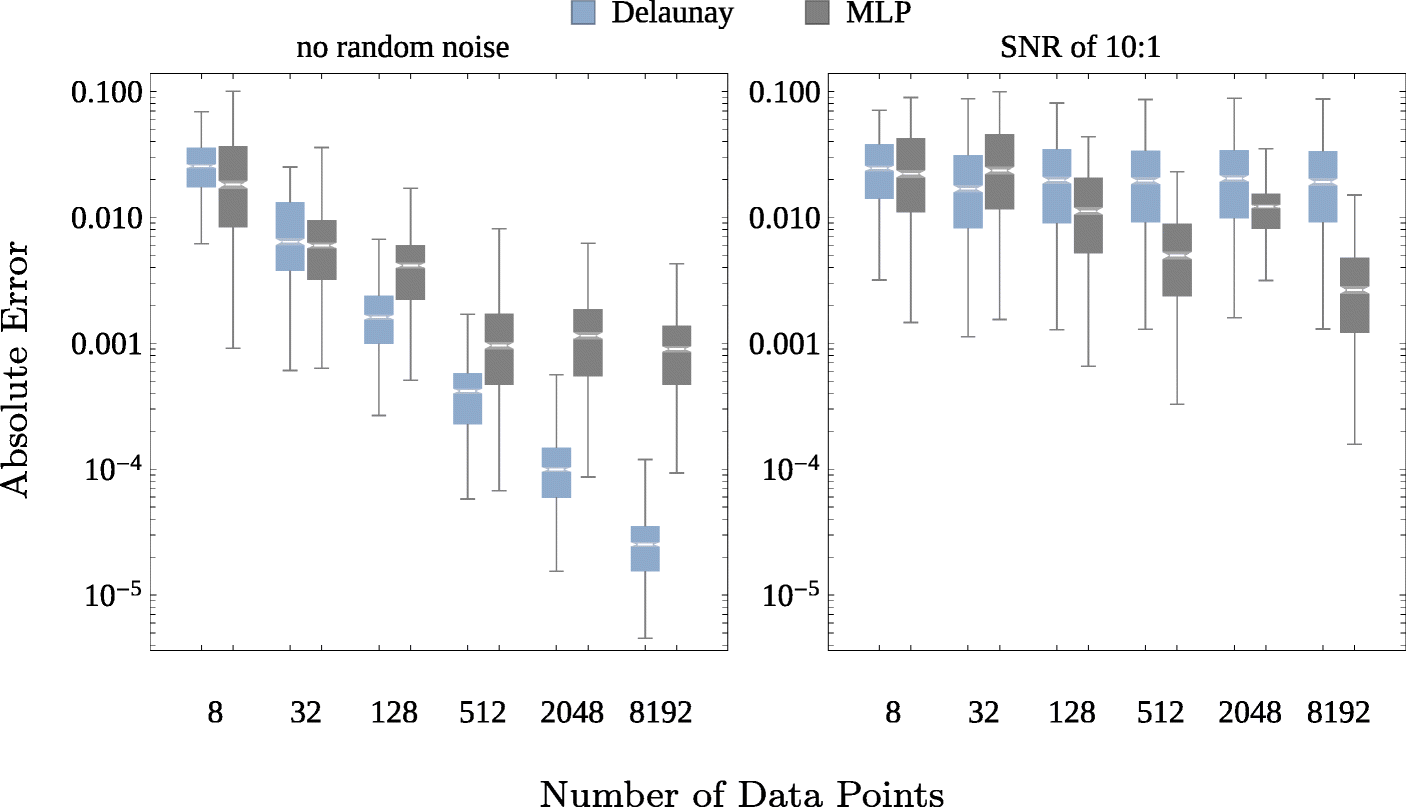
\includegraphics[width=0.7\textwidth]{../img/delaunay_new/2d_errors_w_noise.png}\\
Delaunay interpolation vs MLP error in {\bf 2D} with and w/o noise
\end{center}

\vfill

{\tiny Lux, Watson, Chang, et al.
Interpolation of sparse high-dimensional data.
{\sl Numerical Algorithms 88}, pp.~281–313 (2021).}

\end{frame}

\begin{frame}
\frametitle{The blessing of dimensionality (no noise)}

\begin{center}
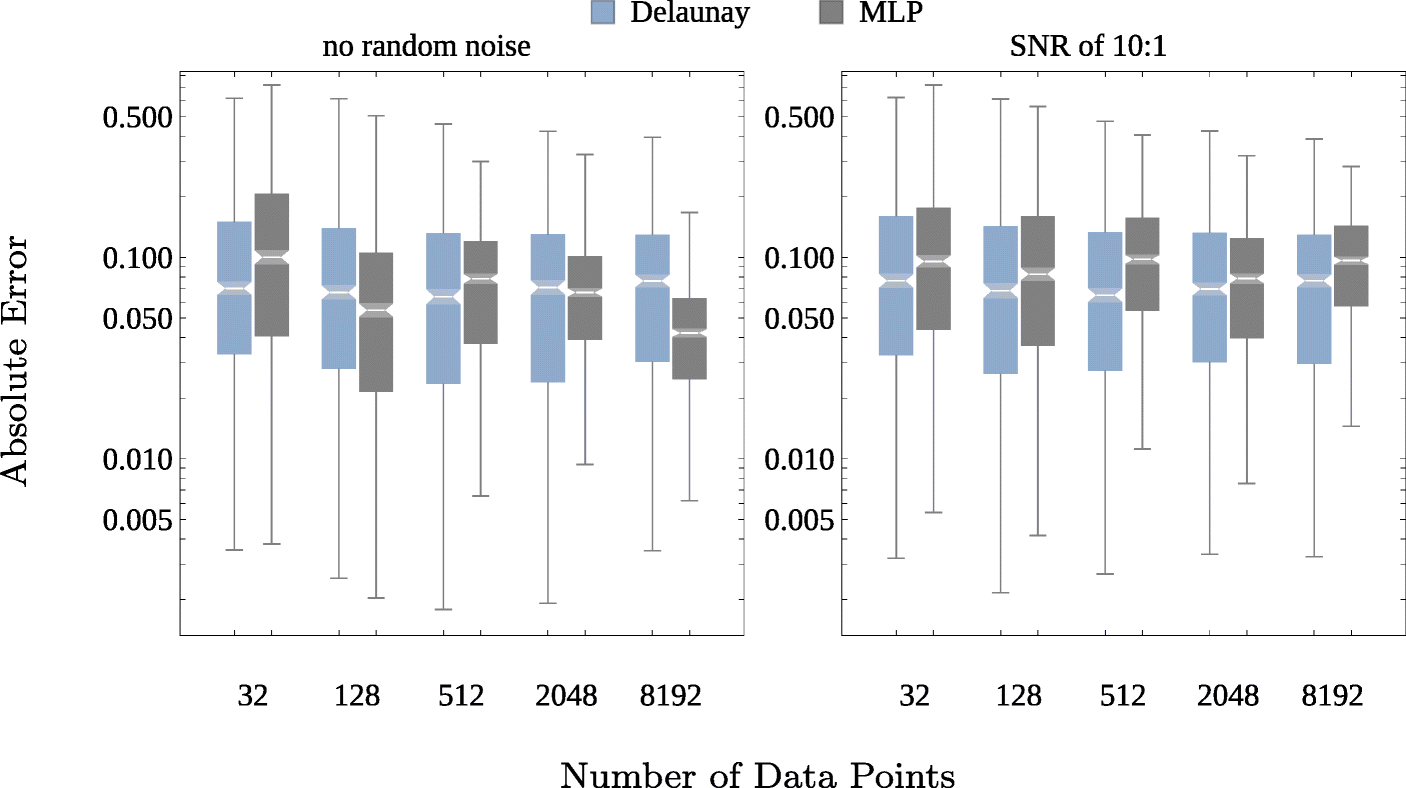
\includegraphics[width=0.7\textwidth]{../img/delaunay_new/20d_errors_w_noise.png}\\
Delaunay interpolation vs MLP error in {\bf 20D} with and w/o noise
\end{center}

\vfill

{\tiny Lux, Watson, Chang, et al.,
Interpolation of sparse high-dimensional data.
{\sl Numerical Algorithms 88}, pp.~281–313 (2021).}

\end{frame}

\begin{frame}
\frametitle{The hopelessness of dimensionality}

Can we still make good predictions where we {\bf do} have data?

\bigskip
\pause

{\bf No, because we have no data anywhere}

\bigskip

We measure where we {\sl might} have enough data to make a prediction
using the ``convex hull'' of the training data $CH({\cal X})$

\bigskip
\pause

If ${\cal X}$ are sampled from {\sl any} distribution,
$\mu(CH({\cal X})) \rightarrow 0$ {\sl exponentially} as $d$ grows

\bigskip

This is called a {\sl concentration of measure}

\vfill

{\tiny Gorban and Tyukin,
Stochastic separation theorems.
{\sl Neural Networks 94}, pp.~255-259 (2017).}

\end{frame}

\begin{frame}
\frametitle{Example}

Suppose that we uniformly sample $x = (x_1, x_2, \ldots, x_d)$ from $[0, 1]^d$

\bigskip

$$
\|x - \frac{1}{2}\|_2^2 = \sum_{i=1}^d{(x_i - \frac{1}{2})^2}.
$$

$$
\mathbb{E}\left[ \left(x_i - \frac{1}{2}\right)^2 \right]
= \int_{0}^1 \left(u - \frac{1}{2}\right)^2 du
= \frac{1}{12}
$$
with finite variance $\nu$

\bigskip

By CLT for all $x \in {\cal X}$:
$\mathbb{E}[\|x - \frac{1}{2}\|_2^2] = \frac{d}{12}$
with variance $\frac{\nu}{d}\rightarrow 0$ as $d\rightarrow\infty$.

\vfill

{\tiny Garg, Chang, and Raghavan,
Stochastic optimization of Fourier coefficiencts to generate space-filling designs.
{\sl To appear in Winter Sim 2023}.}

\end{frame}

\begin{frame}
\frametitle{Hope in problem structure}
\begin{center}
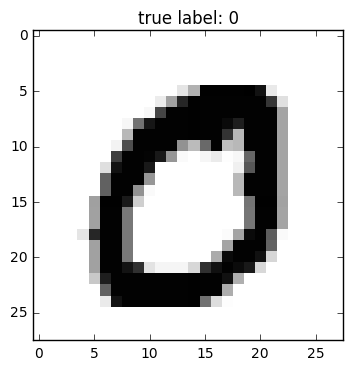
\includegraphics[width=0.1\textwidth]{../img/delaunay_new/mnist_data_0.png}
{\huge $\qquad \xrightarrow{\quad f \quad} \qquad 0$}
\end{center}

\bigskip
$$
28 \times 28 \text{ pixels} \neq 784 \text{ dimensions...}
$$

\end{frame}

\begin{frame}
\frametitle{Modern deep learning pipeline}

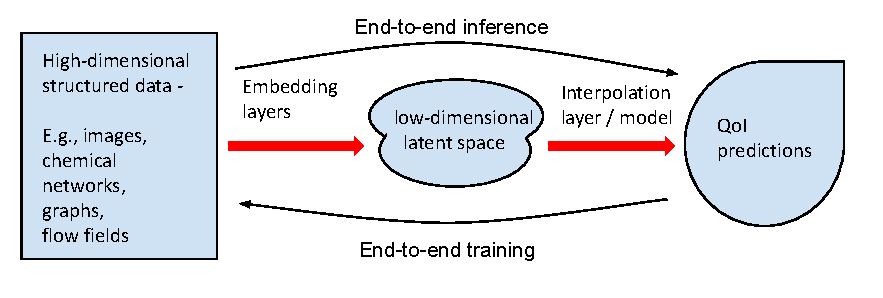
\includegraphics{../img/delaunay_new/interpolating_latent_space.pdf}

\end{frame}

\begin{frame}
\frametitle{Tyler's hot takes on high-dimensional learning}
\begin{itemize}
\pause \item ``Big data'' doesn't exist, all data is small (measure 0)
\pause \item Overfitting is a myth, we can just interpolate
\pause \item SOA deep learning = {\sl representation learning} +
function approximation
\pause \item The ``function approximation'' part is
(piecewise linear) MLP regressors/classifiers
\pause \item Interpolants + approximation theory can give you error bounds,
model validation, interpretablility, and UQ
\end{itemize}
\end{frame}

\begin{frame}
  \frametitle{Outlines}
  \tableofcontents
\end{frame}

\section{High-dimensional interpolation via Delaunay triangulations}

\begin{frame}
\frametitle{Multidimensional piecewise linear interpolation}

To define a piecewise linear interpolant in $\mathbb{R}^d$,
{\bf you need a simplicial mesh over ${\cal X}$}

\begin{columns}
\begin{column}{.62\textwidth}
$\left[x^{(i,0)} \quad \ldots \quad x^{(i,d)} \atop 1 \quad \ldots \quad 1\right]w = \left[q \atop 1\right]$

$$
{\hat f}_{S^{(i)}}(q) = w^T \big(f(x^{(i,0)}), \ldots, f(x^{(i,d)})\big).
$$

\end{column}
\begin{column}{.3\textwidth}
\hbox{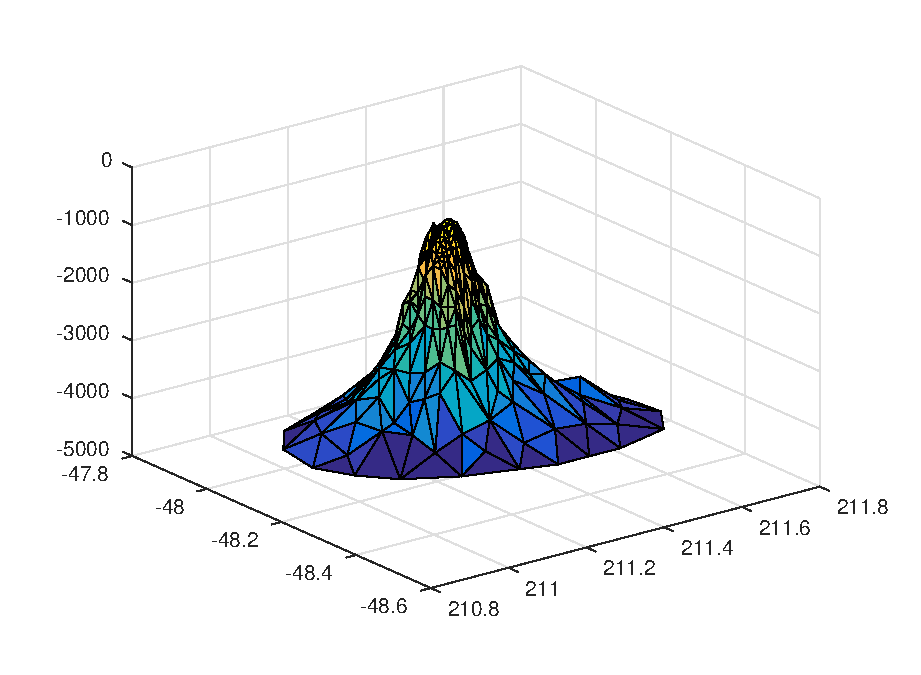
\includegraphics[width=\textwidth]{../img/delaunay_old/seamount.eps}}
\end{column}
\end{columns}

\pause
Taylor bound at $x^{(i,0)}$ is:

$$
\big|f(q) - \hat f(q)\big| \leq \frac{\gamma \|q - x^{(i,0)}\|_{2}^{2}}{2} + \frac{\sqrt{d}  \gamma k^{2}}{2 \sigma_{d}} \|q - x^{(i,0)}\|_{2}.
$$

{\small
$k = \max_{x^{(i,j)} \neq x^{(i,1)}} \|x^{(i,1)} - x^{(i,j)}\|_2$,\\
$\gamma$ is the Lip const of $\nabla f$,\\
$\sigma_d$ is the min singular val of Barycentric interpolation matrix}

\vfill

{\tiny Lux, Watson, Chang, et al.,
Interpolation of sparse high-dimensional data.
{\sl Numerical Algorithms 88}, pp.~281–313 (2021).}

\end{frame}

\begin{frame}{About Delaunay Triangulations}
\begin{itemize}
\item The {\it Delaunay triangulation} ($DT({\cal X})$)
is the ``optimal'' unstructured simplicial mesh of ${\cal X}$
\item {\bf Defining property}:
for all $S \in DT({\cal X})$, the circumball $B^{(S)}$
satisfies
$B^{(S)} \cap {\cal X} = \emptyset$.
\end{itemize}
\begin{center}
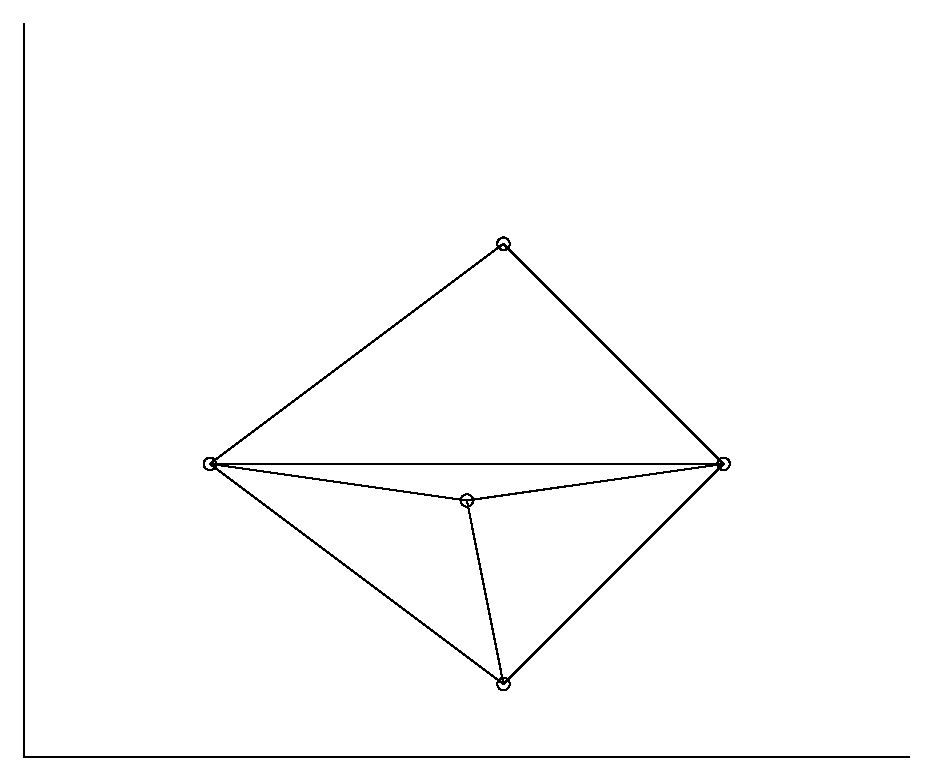
\includegraphics[width=0.25\textwidth]{../img/delaunay_old/triangleplane.eps}
\hskip 4pt{\color{red} \xmark}
$\qquad\qquad$
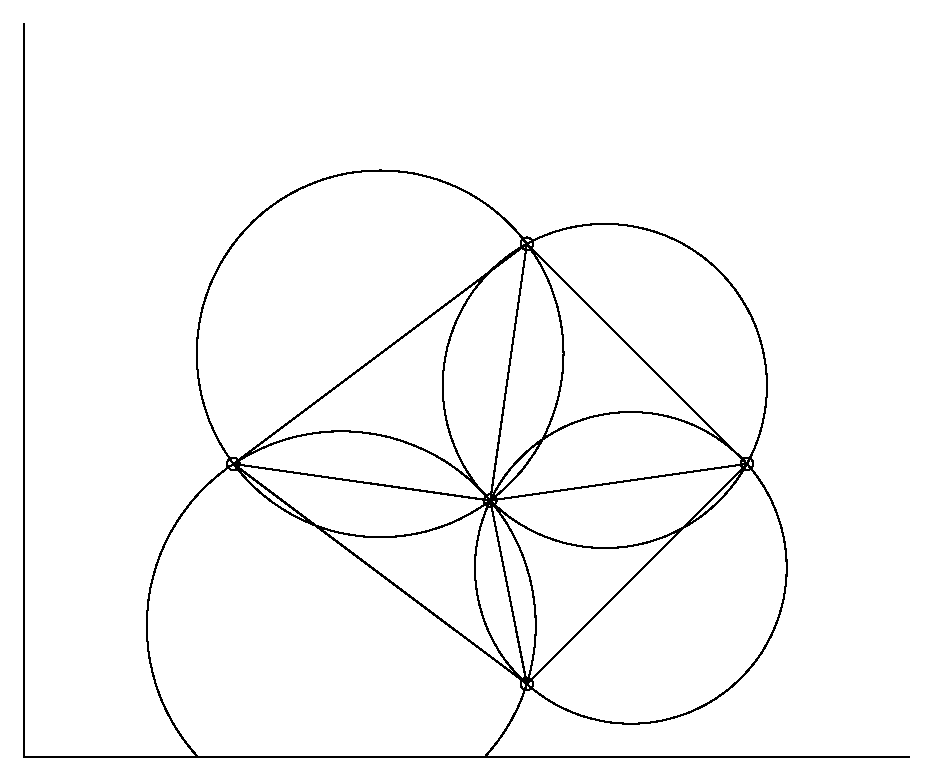
\includegraphics[width=0.25\textwidth]{../img/delaunay_old/delaunayplane.eps}
\hskip 4pt{\color{green} \cmark}
\end{center}
\begin{itemize}
\item $DT({\cal X})$ exists and is unique when ${\cal X}$ is in {\it general position}.
\end{itemize}
\end{frame}

\begin{frame}{Scalability Issues}
\begin{itemize}
\item Meshes blow up exponentially in $d$
\item Oweing to Klee (of Klee-Minty cube fame),
the size of the $DT({\cal X})$ is
$$
\mathcal{O}\left(n^{\lceil d/2 \rceil}\right)
$$
\begin{itemize}
\item For $d > 8$, this is impossible!
\end{itemize}
\end{itemize}
\pause
{\textbf{Observation:}
For a given $q$, we only need vertices
($\{x^{(i,0)}, \ldots, x^{(i,d)}\}$) of $S \in DT({\cal X})$
such that $q\in S$}
$$
{\hat f}_{DT}(q) = \sum_{i=1}^{d+1} w_i\text{~}F(s^{(i)}).
$$
\medskip
\pause
{\textbf{Question:} Can we find $S$ containing $q$ in polynomial time?}
\end{frame}

\section{DelaunaySparse algorithm for high-dimensional interpolation}

% Algorithm for computing the Delaunay interpolant
\begin{frame}{DelaunaySparse Algorithm outline}
Algorithm to locate Delaunay simplex containing $q$:
\begin{itemize}
\item Grow an initial Delaunay simplex (greedy algorithm) that is
``nearby'' to $q$
\item ``Flip'' accross facets from which $q$ is visible to a new Delaunay
simplex (closer to $q$)
\item This ``visibility walk'' converges to $q$ in finite steps
(Edelsbrunner's acyclicity theorem)
\end{itemize}
\vfill
{\tiny Chang et al.,
A polynomial time algorithm for multivariate interpolation in arbitrary
dimension via the Delaunay triangulation.
{\sl In 2018 ACMSE Conf.}}
\end{frame}

\begin{frame}{Algorithm Complexity}
\begin{itemize}
\item To grow the first simplex:
$\mathcal{O}(n d^3)$ to apply $n$ rank-1 updates to the QR factorization of
$d \times j$ matrix for $j=1,\ldots,d$
\item To compute a flip:
$\mathcal{O}(n d^2)$ to apply $n$ rank-1 updates to the QR factorization of
a $d \times d$ matrix
\item $\ell$ total flips\\
\centerline{\small
\begin{tabular}{l|cccc}
  & $n=2K$ & $n=8K$ & $n=16K$ & $n=32K$\\
\hline
$d=2$  & 3.05 & 2.90 & 3.25 & 3.10\\
$d=8$  & 23.75 & 24.75 & 24.30 & 23.10\\
$d=32$ & 95.25 & 125.60 & 131.85 & 150.10\\
$d=64$ & 171.95 & 221.85 & 248.35 & 280.60\\
\end{tabular}}
\end{itemize}
\medskip
\pause
{\bf Overall complexity:} $\mathcal{O}(nd^2 \ell)$\\
\medskip
\pause
{\bf Unresolved question:} $\ell \approx d$? $\ell$ independent of $n$?
\end{frame}

% Linear programming
\begin{frame}{Linear programming interpretation}
$$
{\tilde A} = \left[ \begin{matrix}
(-x^{(1)})^T & 1 \cr
(-x^{(2)})^T & 1 \cr
\vdots & \vdots \cr
(-x^{(n)})^T & 1 \cr
\end{matrix}\right]\text{, }
{\tilde b} = \left[ \begin{matrix}
\| x^{(1)} \|_2^2 \cr
\| x^{(2)} \|_2^2 \cr
\vdots \cr
\| x^{(n)} \|_2^2 \cr
\end{matrix}\right]\text{, and }
{\tilde c} = \left[ \begin{matrix}
-q \cr
1 \cr
\end{matrix}\right].
$$
\pause
$\displaystyle \hbox{\bf Primal prob: }
\max_{\tilde u} {\tilde c}^T {\tilde u}
\hbox{ such that }
{\tilde A}{\tilde u} \leq {\tilde b}, {\tilde u}\hbox{ free}.$\\
{\bf Ext pts:}
${\tilde u} = (-2\hbox{circumcenter}, \hbox{circumradius}^2 - \|\hbox{circumcenter}\|_2^2)$\\
\medskip
\pause
$\displaystyle \hbox{\bf Dual prob: }
\min_{\tilde v} {\tilde b}^T {\tilde v}
\hbox{ such that }
{\tilde A}^T{\tilde v} = {\tilde c}, {\tilde v}\geq 0.$\\
{\bf Ext pts:}
$\Rightarrow$ ${\tilde v}$ are convex weights for $q$\\
\medskip
\pause
Primal + dual feasible $\Rightarrow$ Delaunay simplex containing $q$\\
\medskip
\pause
{\bf LP basic solution in polynomial time is an open problem!}
\end{frame}

% Extrapolation
\begin{frame}{Extrapolation}
What about extrapolation?
\begin{itemize}
\item Project $q$ on to the convex hull of ${\cal X}$
\item Interpolate the projection (if the residual is small)
\item Projection is a quadratic program
\end{itemize}
Let $E$ be a $d\times n$ matrix whose columns are points in ${\cal X}$, and let
$z$ be an extrapolation point (outside convex hull of ${\cal X}$).
$$
\xi^* = \arg\min_{\xi\in\mathbb{R}^n} \|E\xi - z\| \quad\hbox{subject to}\quad
\xi \ge 0 \quad\hbox{and}\quad \sum_{i=1}^n \xi_i = 1.
$$
Projection: ${\hat z} = E\xi^*$

\vfill

{\tiny Chang et al.,
Remark on Algorithm 1012.
{\sl In preparation}.}
\end{frame}

% DELAUNAYSPARSE
\begin{frame}{DELAUNAYSPARSE Package}
Standalone software package {\tt DELAUNAYSPARSE}:
\begin{columns}
\begin{column}{.5\textwidth}
\begin{itemize}
\item Robust against degeneracy
\item Runs in $\mathcal{O}(m n d^2 \ell)$ time
\end{itemize}
\end{column}
\begin{column}{.5\textwidth}
\begin{itemize}
\item Parallel and serial implementations
\end{itemize}
\end{column}
\end{columns}
\begin{columns}
\begin{column}{.15\textwidth}
Runtime (secs) for interpolating a single $q$
\end{column}
\begin{column}{.8\textwidth}
{\small
\begin{center}
\begin{tabular}{c|rrrrr}
& & & $d\quad$ & & \\
$n$ & $2\quad$ & $8\quad$ & $32\quad$ & $64\quad$ & $128\quad$ \\
\hline
250    & 0.005  & 0.013   & 0.150   & 3.404    & 27.078   \\
500    & 0.021  & 0.042   & 0.325   & 6.479    & 59.511   \\
1000   & 0.083  & 0.152   & 0.791   & 14.020   & 124.320  \\
2000   & 0.344  & 0.583   & 2.230   & 28.984   & 242.066  \\
4000   & 1.314  & 2.284   & 7.165   & 62.494   & 502.620  \\
8000   & 5.580  & 9.027   & 26.210  & 151.177  & 905.711  \\
16,000 & 22.086 & 35.725  & 109.448 & 386.596  & 2190.362 \\
32,000 & 82.915 & 145.115 & 421.934 & 1097.060 & 5024.675 \\
\end{tabular}
\end{center}
}
\end{column}
\end{columns}
\vfill
{\tiny Chang et al.,
Algorithm 1012: DELAUNAYSPARSE.
{\sl ACM TOMS 46(4)}, Article No.~28 (2020).}
\end{frame}

\section{Preliminary Results and Future Work}

\begin{frame}
\frametitle{Recall...}

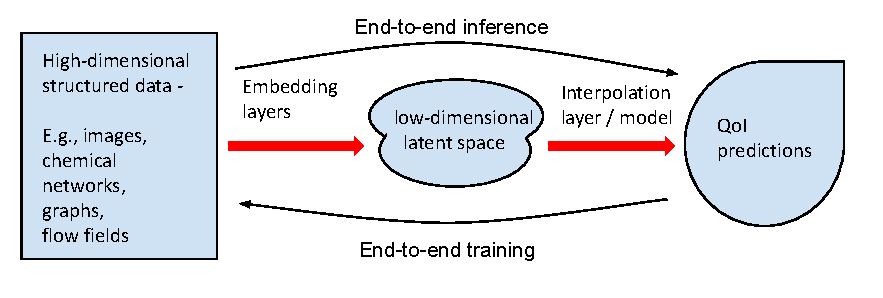
\includegraphics{../img/delaunay_new/interpolating_latent_space.pdf}

\end{frame}

\begin{frame}
\frametitle{Early results on Airfoil Predictions}

Thanks to Romit for providing airfoil prediction data,
dimension reduced from 100,000+  down to {\bf 8D} via autoencoder


Delaunay interpolation in latent space

\medskip

\begin{center}
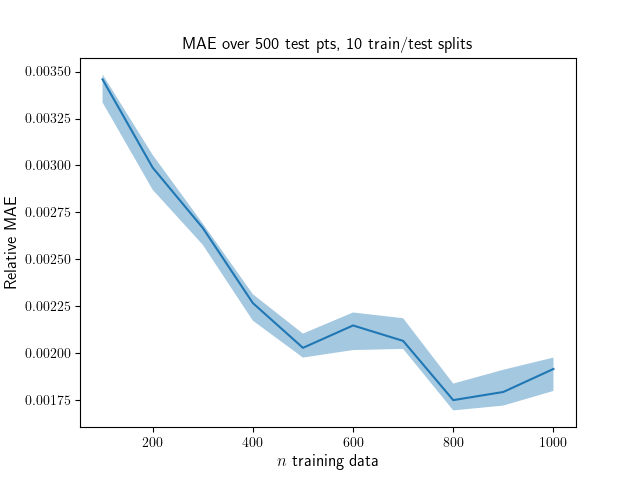
\includegraphics[width=0.48\textwidth]{../img/delaunay_new/latent_delaunay_lift.png}
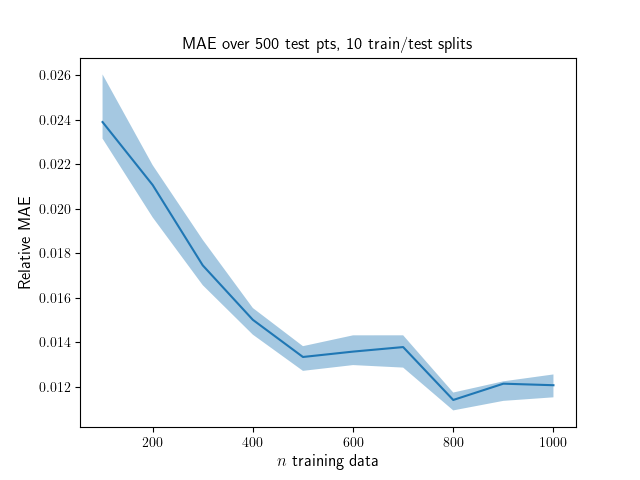
\includegraphics[width=0.48\textwidth]{../img/delaunay_new/latent_delaunay_drag.png}\\
$\quad$Lift predictions $\qquad\qquad\qquad\qquad\qquad$ Drag predictions
\end{center}

\end{frame}

\begin{frame}
\frametitle{But what do you get?}

\begin{itemize}
\pause\item {\bf Interpretability:}
\begin{itemize}
\item These $d+1$ training points were used in this prediction
\item Simplex is ill-conditioned, need more data in this direction
\end{itemize}
\pause\item {\bf Verifiability:}
\begin{itemize}
\item Do the results agree with the error bounds?
\item See preprint on Delaunay Diagnostic from LLNL
\end{itemize}
\pause\item {\bf Error bounds and UQ:}
\begin{itemize}
\item Coming soon...
\end{itemize}
\end{itemize}

\vfill

{\tiny Gillette and Kur,
Data-driven geometric scale detection via Delaunay interpolation.
{\sl arXiv preprint 2203.05685.}}

{\tiny
Chang, Gillette, and Maulik, {\sl in preparation}.
}

\end{frame}

\begin{frame}
\frametitle{Next steps}

\onslide<1>{
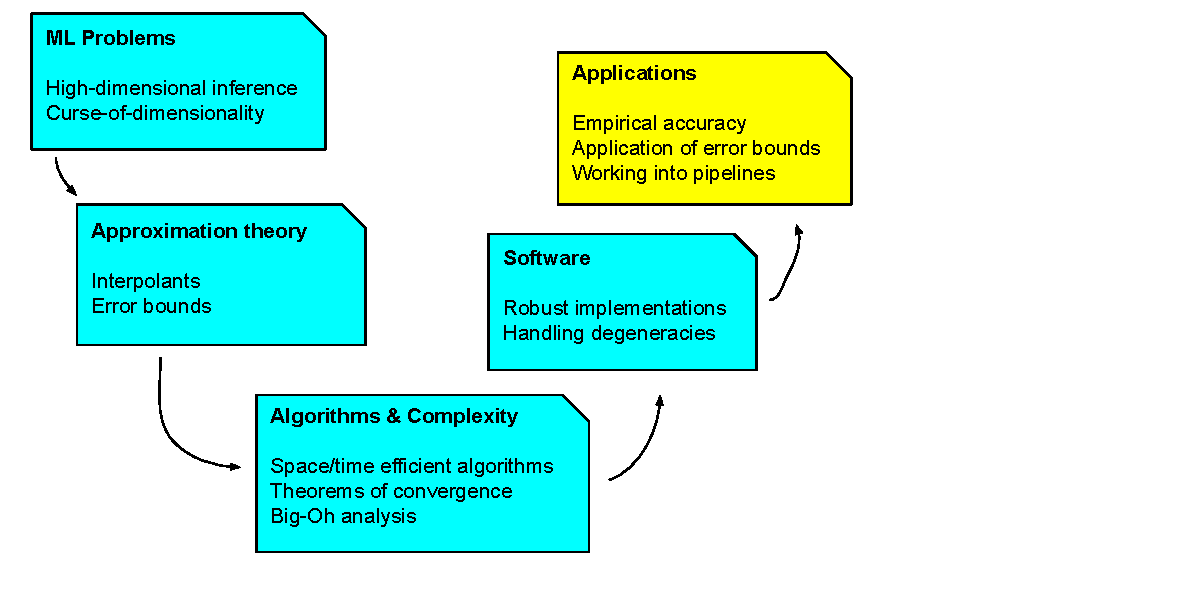
\includegraphics[width=\textwidth]{../img/delaunay_new/ToDo0.pdf}}

\onslide<2>{
\vskip -18.5em
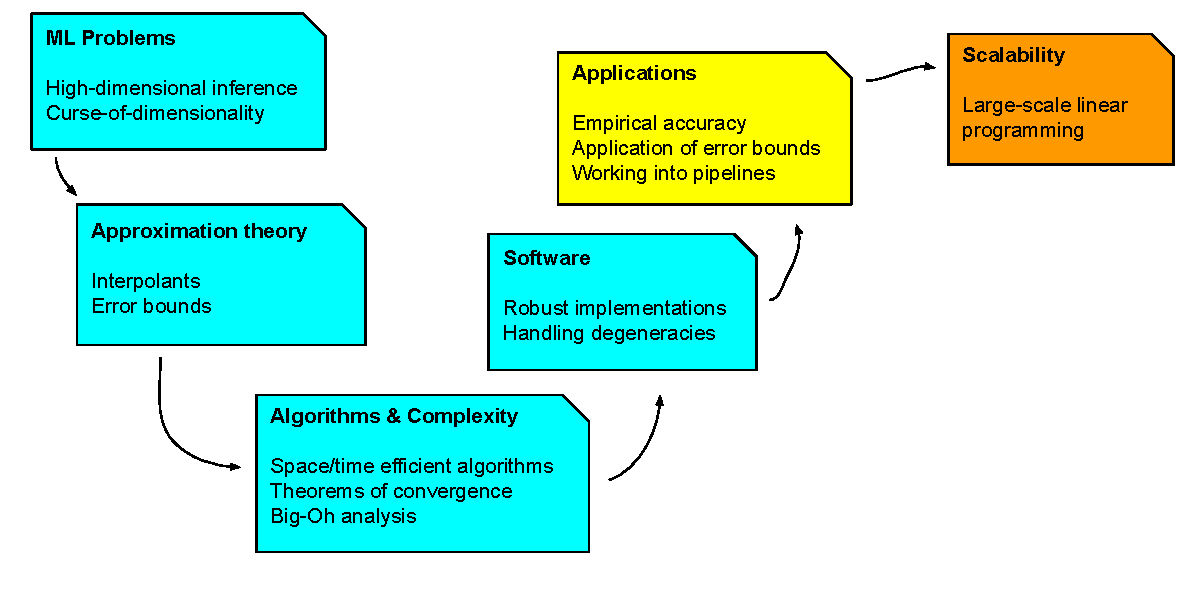
\includegraphics[width=\textwidth]{../img/delaunay_new/ToDo1.pdf}}

\onslide<3>{
\vskip -18.5em
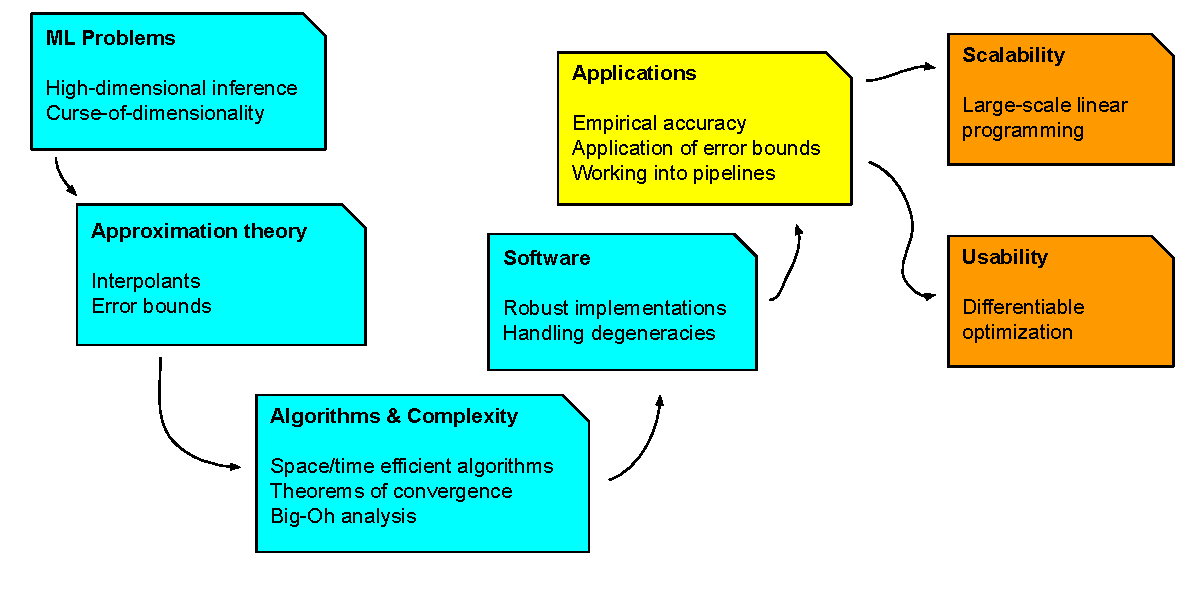
\includegraphics[width=\textwidth]{../img/delaunay_new/ToDo2.pdf}}

\onslide<4>{
\vskip -18.5em
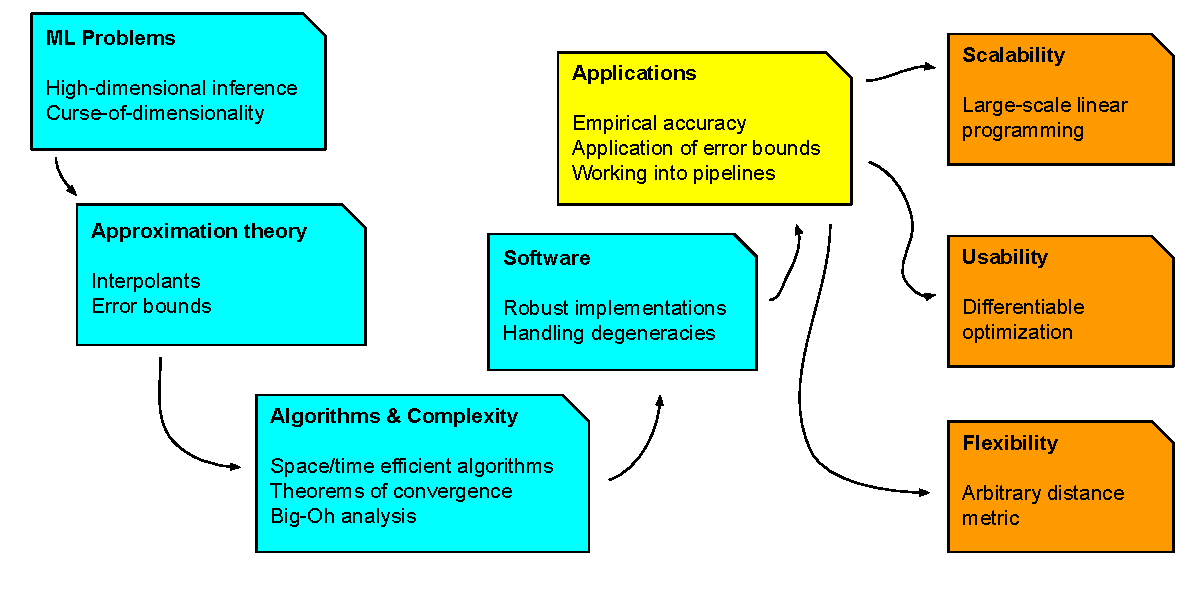
\includegraphics[width=\textwidth]{../img/delaunay_new/ToDo3.pdf}}

\end{frame}

\begin{frame}
\frametitle{Acknowledgements}

This work was supported in part by the VarSys project:
NSF Grants CNS-1565314 and CNS-1838271.

\bigskip

This work was also supported in part by FASTMath Institute:
U.S.~Department of Energy,
Office of Science, Office of Advanced Scientific Computing Research,
SciDAC program under contract number DE-AC02-06CH11357.

\end{frame}

\begin{frame}
  \frametitle{Questions}
  \tableofcontents
  \bigskip
\end{frame}

% Delaunay graph appendics
\section{Bonus Slides: Computing the Delaunay Graph}

\begin{frame}{The Delaunay Graph}
\begin{itemize}
\item Delaunay graph of ${\cal X} = DG({\cal X})$
\item Connect 2 vertices iff they are shared by a single Delaunay simplex
\item Used for:
\begin{itemize}
\item Neighbor structure in spatial data
\item Topological shape analysis
\end{itemize}
\item There are at most $n(n-1)/2$ edges
\item Current state-of-the-art implementation in CGAL computes $DG({\cal X})$ from
$DT({\cal X})$ -- scales well for large $n$, infeasible for $d\geq10$
\end{itemize}
\end{frame}

\begin{frame}{Getting the Delaunay Graph}
\begin{itemize}
\item The number of connections in $DG({\cal X})$ is upper bounded by $n(n-1)/2$
\item Can recover $DG({\cal X})$ by interpolating the midpoint between each
pair of points in ${\cal X}$
\begin{itemize}
\item If the simplex containing the midpoint between $x^{(1)}$ and $x^{(2)}$
also contains both $x^{(1)}$ and $x^{(2)}$, then they are clearly connected
\item If not, then it certifies that they are not connected in {\it a}
Delaunay triangulation (in case degenerate)
\end{itemize}
\item Using {\tt DELAUNAYSPARSE}, requires
$\mathcal{O}(n^3 d^2 \ell)$ time --- better than current state-of-the-art for
$d$ large, worse for $n$ large
\end{itemize}

\vfill

{\tiny Full proof in my PhD dissertation:

Chang, {\sl Mathematical Software for Multiobjective Optimization Problems}.
PhD dissertation, Virginia Tech (2020).
}
\end{frame}

\begin{frame}
\frametitle{Parallel scaling}

For $d>8$, CGAL crashes with out-of-memory error

\begin{center}
\includegraphics[width=0.7\textwidth]{../img/delaunay_new/parallel_scaling_plot.eps}
\end{center}

\vfill

\pause Paper has been rejected due to lack of real-world data
\end{frame}
\end{document}
